\begin{frame}{My Research}
\begin{itemize}
    \item \small {\textit{Polyanya} only work for single pair shortest path}
    \item My research:
        \begin{itemize}
            \item \small{multi-targets search based on framework of \textit{Polyanya}}
            \item \small{with good scalability}
        \end{itemize}
\end{itemize}
\end{frame}

\begin{frame}{Multi-target Search: interval heuristic}
\begin{minipage}{.6\textwidth}
\begin{itemize}
\item \small {Let's review heuristic function in \textit{Polyanya}}
    \begin{itemize}
        \item \small{
            \textit{g-value}: depends on previous search and current root
        }
        \item \small{
            \textit{h-value}: depends on current search node and given target
        }
    \end{itemize}
\item \small how about remove $t$ from \textit{h-value}?
\end{itemize}
\end{minipage}%
\begin{minipage}{.4\textwidth}
    \begin{adjustbox}{max totalsize={.9\textwidth}{.9\textheight}, right}
    \begin{tikzpicture}
        \coordinate (a) at (2, 5);
\coordinate (b) at (5, 2);
\coordinate (r) at (2, 3);
\coordinate (t1) at (5, 4);
\coordinate (t2) at (2, 6);
\coordinate (t3) at (3, 2);
\coordinate (q) at (1, 1);

\newcommand{\nodelabel}[2] {
    \node[fill,circle,scale=0.2,label=#2:$#1$,color=red] at (#1) {$#1$};
}

\newcommand{\drawST}[2] {
    \node[fill,circle,scale=0.2,label=#2:$#1$,color=blue] at (#1) {$#1$};
}

\newcommand{\snode}{
    \draw [gray] (a)--(b);
    \drawST{q}{right}
    \drawST{t1}{above}
    \nodelabel{r}{below}
    \nodelabel{a}{above}
    \nodelabel{b}{above}
}

\newcommand{\gvalue}{
    \draw [->,black, very thick] (q.north) to [out=30,in=150] (r.north);
}

\newcommand{\hvalue}{
    \draw[black,dashed,very thick] (r)--(t1);
}
        \onslide<1->{\snode}
        \onslide<2>{\gvalue}
        \onslide<3->{\hvalue}
    \end{tikzpicture}
    \end{adjustbox}
\end{minipage}
\end{frame}

\begin{frame}{Multi-target Search: interval heuristic}
\begin{minipage}{.6\textwidth}
Then we get: Interval heuristic
\begin{itemize}
    \item \textit{g-value} is same
    \item \textit{h-value}: distance from $r$ to $I$
\end{itemize}
\end{minipage}%
\begin{minipage}{.4\textwidth}
    \begin{adjustbox}{max totalsize={.9\textwidth}{.9\textheight}, right}
    \begin{tikzpicture}
        \coordinate (a) at (2, 5);
\coordinate (b) at (5, 2);
\coordinate (r) at (2, 3);
\coordinate (t1) at (5, 4);
\coordinate (t2) at (2, 6);
\coordinate (t3) at (3, 2);
\coordinate (q) at (1, 1);

\newcommand{\nodelabel}[2] {
    \node[fill,circle,scale=0.2,label=#2:$#1$,color=red] at (#1) {$#1$};
}

\newcommand{\drawST}[2] {
    \node[fill,circle,scale=0.2,label=#2:$#1$,color=blue] at (#1) {$#1$};
}

\newcommand{\snode}{
    \draw [gray] (a)--(b);
    \drawST{q}{right}
    \drawST{t1}{above}
    \nodelabel{r}{below}
    \nodelabel{a}{above}
    \nodelabel{b}{above}
}

\newcommand{\gvalue}{
    \draw [->,black, very thick] (q.north) to [out=30,in=150] (r.north);
}

\newcommand{\hvalue}{
    \draw[black,dashed,very thick] (r)--(t1);
}
        \hivalue
    \end{tikzpicture}
    \end{adjustbox}
\end{minipage}
\end{frame}

\begin{frame}{Multi-target Search: target heuristic}
\begin{minipage}{.6\textwidth}
\begin{itemize}
    \item \small{
        \textit{interval heuristic} causes redundant expansions
    }
    \item \small{
        especially in sparse targets scenario
    }
    \item \small{
        e.g.: query is "nearest storage locations where capacity $>=100$".
    }
\end{itemize}
\end{minipage}%
\begin{minipage}{.4\textwidth}
    \begin{adjustbox}{max totalsize={.9\textwidth}{.9\textheight}, right}
    \begin{tikzpicture}
        \newcommand{\nodelabel}[2] {
    \fill[red] (#1) circle[radius=.5ex];
    \node[#2] at (#1) {#1};
}

\newcommand{\medge}[2]{
    \draw[gray,thick] (#1)--(#2);
}

\newcommand{\drawVs}{
    %\nodelabel{a}{above}
    \nodelabel{b}{below}
    \nodelabel{c}{below}
    
    %\nodelabel{d}{left}
    \nodelabel{e}{right}
    \nodelabel{f}{below}
    
    \nodelabel{g}{above}
    \nodelabel{h}{below}
    %\nodelabel{i}{below}
}

\newcommand{\drawmeshs}{
    \medge{a}{k},\medge{a}{d},\medge{a}{b},\medge{a}{c}
    \medge{b}{c},
    \medge{c}{g}
    \medge{d}{f},\medge{d}{l},\medge{d}{e}
    \medge{l}{f}
    \medge{e}{c},\medge{e}{f}
    \medge{f}{h}
    \medge{g}{h},\medge{g}{b}
    \medge{h}{i}
}

\newcommand{\drawobstacles}{
    \fill[black] (a)--(b)--(c)--cycle;
    \fill[black] (g)--(h)--(i)--cycle;
    \fill[black] (d)--(e)--(f)--cycle;
}

%\coordinate (a) at (2, 6); 
\coordinate (a) at (0, 7);
\coordinate (b) at (8, 7); 
\coordinate (c) at (6, 5); 
\coordinate (d) at (1, 3);
\coordinate (e) at (4, 3);
\coordinate (f) at (4, 2);
\coordinate (g) at (7, 4);
\coordinate (h) at (7, 2);
%\coordinate (i) at (9, 0);
\coordinate (i) at (10, 0);
\coordinate (j) at (5, 2);
\coordinate (k) at (0, 7);
\coordinate (l) at (0, 0);
\coordinate (m) at (10, 0);
\coordinate (n) at (10, 7);
\coordinate (q) at (3, 4);
\coordinate (t) at (9, 3); 
% boundary
\draw[black, ultra thick] (k)--(n)--(m)--(l)--cycle;

% obstacles
\drawobstacles
% mesh
\drawmeshs
% vertices
\drawVs
% start
\fill[blue] (q) circle[radius=.5ex];
\node[above] at (q) {$q$};
% end
\fill[blue] (t) circle[radius=.5ex];
\node[above] at (t) {$t$};
        \intervalexpansion
    \end{tikzpicture}
    \end{adjustbox}
\end{minipage}
\end{frame}


\begin{frame}{Multi-target Search: target heuristic}
\begin{minipage}{.6\textwidth}
\small{Introduce the detail of \textit{h-value} in \textit{Polyanya},\\
$h_p(node, t)$ is}:
\begin{itemize}
    \item \small{
        Case 1: $d_e(r, t_1)$
    }
    \item \small{
        Case 2: $d_e(r, a) + d_e(a, t_2)$\\
         or $d_e(r, b) + d_e(b, t_2)$
    }
    \item \small{
        Case 3: when $r$ and $t_3$ at same side, compute mirror point of $t_3$, and go to Case 1 or Case 2
    }
\end{itemize}

\end{minipage}%
\begin{minipage}{.4\textwidth}
    \begin{adjustbox}{max totalsize={.9\textwidth}{.9\textheight}, right}
    \centering
    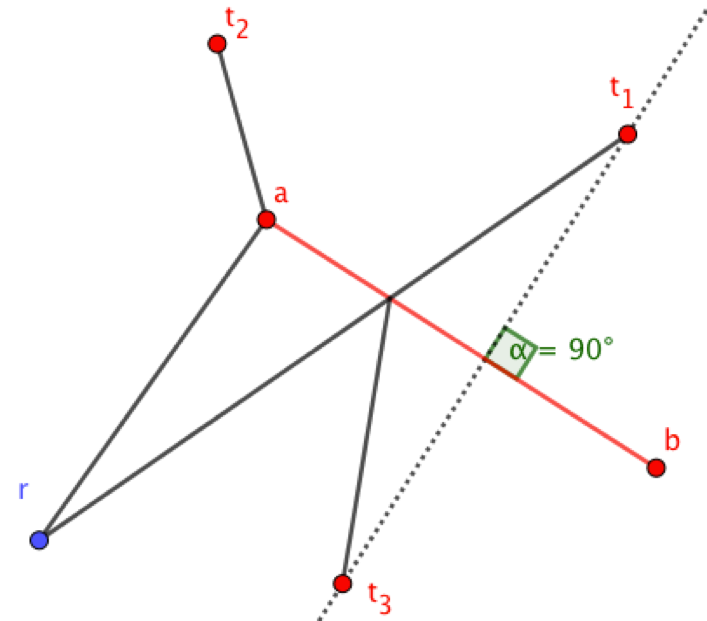
\includegraphics{pic/ef.png}
    \end{adjustbox}
\end{minipage}
\end{frame}

\begin{frame}{Multi-target Search: target heuristic}
\setbeamercovered{invisible}
\begin{minipage}{\textwidth}
\small{
When there are multiple targets ...
}
\onslide<2>{
    \begin{definition}{closest target of search node}
    is a target $t$ that $h_p(node, t)$ is minimal.
    \end{definition}
}
\end{minipage}%
\end{frame}

\begin{frame}{Multi-target Search: target heuristic}
\begin{minipage}{.4\textwidth}
\small{
    How to find the closest target for a search node?
}
\begin{itemize}
    \item<2-> \small{Let $NN_e$ be traditional nearest neighbor in euclidean space}
    \item<3-> \small{It must be:}
    \begin{itemize}
        \item<4-> $NN_e(areaA, a)$ or
        \item<5-> $NN_e(areaB, b)$ or
        \item<6-> $NN_e(areaC, r)$ or
        \item<7-> $NN_e(areaC', r')$ or
    \end{itemize}
    \item<8-> Standard \textit{R-tree} query
\end{itemize}

\end{minipage}%
\begin{minipage}{.6\textwidth}
    \begin{adjustbox}{max totalsize={.9\textwidth}{.9\textheight}, right}
    \centering
    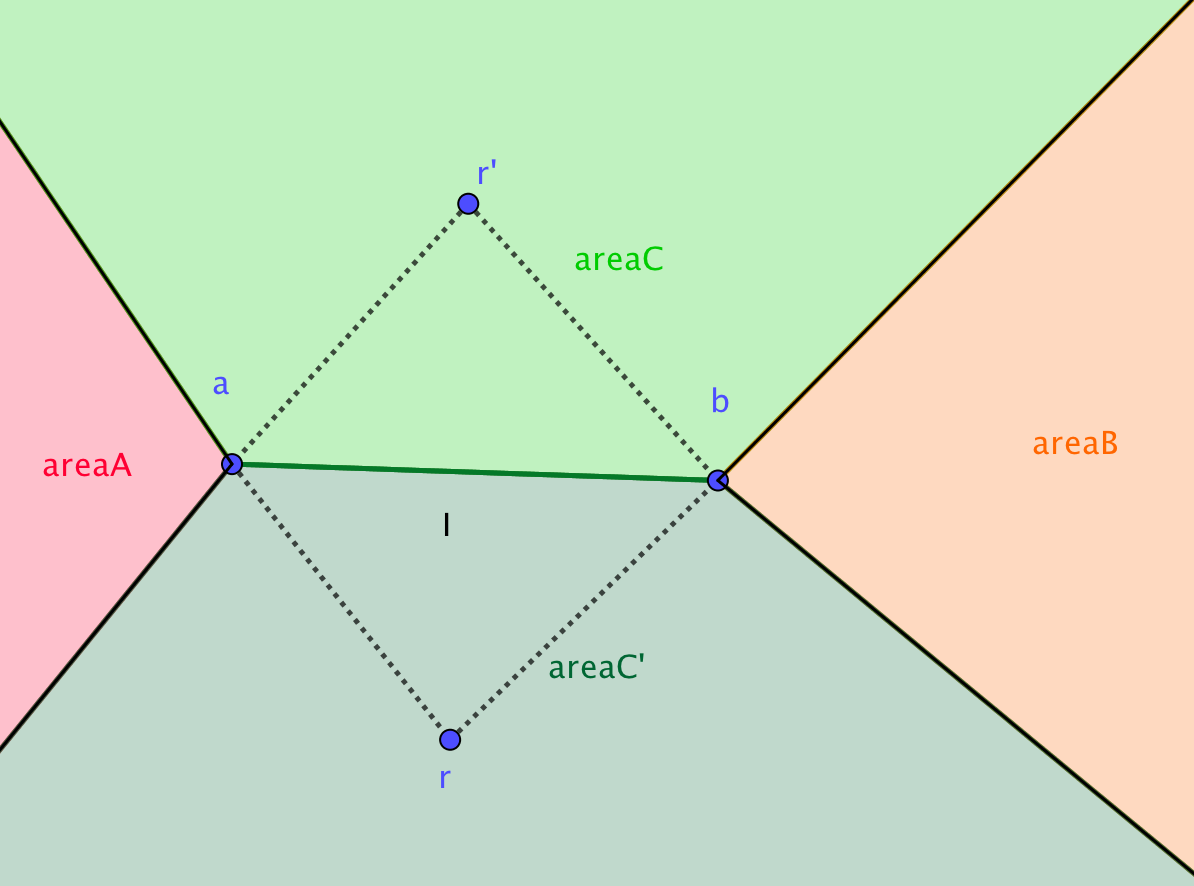
\includegraphics{pic/heuristic.png}
    \end{adjustbox}
\end{minipage}
\end{frame}

\begin{frame}{Multi-target Search: target heuristic}
\begin{minipage}{.9\textwidth}
\begin{itemize}
    \onslide<1-> \item \small{
        For each successor, assign the closest target to it
    }
    \onslide<2-> \item \small {
    Correctness:
    \begin{lemma}{Non-decreasing property:}
        Whenever the closest target of a search node changes,
        the \textit{h-value} never decrease.
    \end{lemma}
    }
\end{itemize}
\end{minipage}%
\end{frame}

\begin{frame}{Multi-target Search: target heuristic}
\setbeamercovered{invisible}
\begin{minipage}{.9\textwidth}
\begin{itemize}
    \item \small{Four \textit{R-tree} queries for each search  node is expensive}
    \item \small{So we are looking for further refinements...}
\end{itemize}
\end{minipage}%
\end{frame}

\begin{frame}{Multi-target Search: target heuristic refinements}
\setbeamercovered{invisible}
\begin{minipage}{.9\textwidth}
\begin{itemize}
    \item \small{Lazy query}
    \begin{Definition}
        In expansion, instead of finding a new target, successors can inherit the closest target from their parent if the \textit{h-value} doesn't change.
    \end{Definition}
    \item \small{Correctness}
    \begin{lemma}
        In this case, it is impossible to find a target with less \textit{h-value}.
    \end{lemma}
\end{itemize}
\end{minipage}%
\end{frame}

\begin{frame}{Multi-target Search: target heuristic refinements}
\setbeamercovered{invisible}
\begin{minipage}{.9\textwidth}
\begin{itemize}
    \item \small{Reassignment}
    \begin{definition}
        \small Once $t$ be retrieved, we must reassign another target to those search nodes who are regarding $t$ as their closest target
    \end{definition}
    \item \small{Lazy reassignment}
    \begin{definition}
        \small Instead of exploring the entire open list, we can do reassignment when such search node pop out
    \end{definition}
    \item \small{Correctness}
    \begin{lemma}
        \small Lazy reassignment doesn't change relative expansion order.
    \end{lemma}
\end{itemize}
\end{minipage}%
\end{frame}